\documentclass[12pt]{article}

\usepackage{amsmath}
\usepackage{amsfonts}
\usepackage{float}
\usepackage{fancyhdr}
\usepackage{graphicx}
\usepackage[colorlinks=true,linkcolor=blue, citecolor=red]{hyperref}
\usepackage{url}
\usepackage[top=.75in, left=.75in, right=.75in, bottom=1in]{geometry}
\usepackage[utf8]{vietnam}

% For algorithm
\usepackage{algorithm}
\usepackage{algpseudocode}

% ============ CODE ============
\usepackage{listings}
\usepackage{xcolor}
\definecolor{codegreen}{rgb}{0,0.6,0}
\definecolor{codegray}{rgb}{0.5,0.5,0.5}
\definecolor{codepurple}{rgb}{0.58,0,0.82}
\definecolor{backcolour}{rgb}{0.95,0.95,0.92}

% Styling for the code.
\lstdefinestyle{mystyle}{
    backgroundcolor=\color{backcolour},   
    commentstyle=\color{codegreen},
    keywordstyle=\color{magenta},
    numberstyle=\tiny\color{codegray},
    stringstyle=\color{codepurple},
    basicstyle=\ttfamily\footnotesize,
    breakatwhitespace=false,         
    breaklines=true,                 
    captionpos=b,                    
    keepspaces=true,                 
    numbers=left,                    
    numbersep=5pt,                  
    showspaces=false,                
    showstringspaces=false,
    showtabs=false,                  
    tabsize=2
}
\lstset{style=mystyle}

% Disable indentation on new paragraphs
\setlength{\parindent}{0pt}

% Optional: graphic path
% \graphicspath{PATH_TO_GRAPHIC_FOLDER}

% To use Times font family, uncomment this row
% \usepackage{mathptmx}

% To use roman section / subsection, uncomment these rows
% \renewcommand{\thesection}{\Roman{section}}
% \renewcommand{\thesubsection}{\thesection.\Roman{subsection}}

% Define course name, report name and report title.
\newcommand{\coursename}{Nhập môn lập trình}
\newcommand{\reportname}{Game Caro}
\newcommand{\reporttitle}{Báo cáo Đồ án - Nhóm 5}

\newcommand{\studentname}{Đinh Đức Anh Khoa   (23122001)\\Nguyễn Lê Hoàng Trung (23122002)\\Nguyễn Đình Hà Dương (23122004)\\Đinh Đức Tài (23122013)}
\newcommand{\teachername}{TS. Trương Toàn Thịnh}

\newcommand{\leftfooter}{\LaTeX\ by \href{https://www.facebook.com/ductai.05/}{Dinh Duc Tai}}

% ============ HEADER AND FOOTER ============
% Header length
\setlength{\headheight}{29.43912pt}

% Footer page number would be on the lower-right corner
\pagestyle{fancy}
\fancyfoot{}
\fancyfoot[R]{Trang \thepage}

\lhead{\reporttitle}
\rhead{
Trường Đại học Khoa học Tự nhiên - ĐHQG HCM\\
\coursename
}
\lfoot{\leftfooter}

% ============ DOCUMENT ============
\begin{document}
\begin{titlepage}
\newcommand{\HRule}{\rule{\linewidth}{0.5mm}}
\centering

\textsc{\LARGE đại học quốc gia tphcm}\\[1.5cm]
\textsc{\Large trường đại học khoa học tự nhiên}\\[0.5cm]
\textsc{\large khoa công nghệ thông tin}\\[0.5cm]
\textsc{bộ môn công nghệ tri thức}\\[0.5cm]

\HRule \\[0.4cm]
{ 
\huge{\bfseries{\reporttitle}}\\[0.5cm]
\large{\bfseries{Đề tài: \reportname}}
}\\[0.4cm]
\HRule \\[0.5cm]

\textbf{\large Môn học: \coursename}\\[0.5cm]

\begin{minipage}[t]{0.4\textwidth}
\begin{flushleft} \large
\emph{Sinh viên thực hiện:}\\
\studentname
\end{flushleft}
\end{minipage}
~
\begin{minipage}[t]{0.4\textwidth}
\begin{flushright} \large
\emph{Giáo viên hướng dẫn:} \\
\teachername
\end{flushright}
\end{minipage}\\[2cm]

{\large \today}\\[2cm]


\includegraphics[scale=.25]{img/hcmus-logo.png}\\[1cm] 

\vfill
\end{titlepage}
	
	
\tableofcontents
\pagebreak

\section{Giới thiệu}
\paragraph{Đây là bài báo cáo Đồ án CARO, môn Nhập môn lập trình.\\ Đồ án CARO được thực hiện bởi nhóm 5, gồm các thành viên:}

\begin{itemize}
    \item Đinh Đức Anh Khoa (23122001)
    \item Nguyễn Lê Hoàng Trung (23122002)
    \item Nguyễn Đình Hà Dương (23122004)
    \item Đinh Đức Tài (23122013)
\end{itemize}
\section{Phân công nhiệm vụ}

Sau đây là bảng phân công nhiệm vụ cho từng thành viên:

\begin{table}[H]
\begin{tabular}{|l|l|l|l|l}
\cline{1-4}
Họ và tên & MSSV & Chức vụ & Nhiệm vụ &  \\ \cline{1-4}
Đinh Đức Anh Khoa & 23122001 & \multicolumn{1}{c|}{Nhóm trưởng} & \begin{tabular}[c]{@{}l@{}}- Phát triển tính năng, xây dựng \\    cấu trúc chương trình.\\ - Xây dựng thuật toán cốt lõi của game.\end{tabular} &  \\ \cline{1-4}
Nguyễn Đình Hà Dương & 23122002 & Thành viên & \begin{tabular}[c]{@{}l@{}}- Thiết kế đồ họa, hình ảnh\\ - Làm trình chiếu PowerPoint\end{tabular} &  \\ \cline{1-4}
Nguyễn Lê Hoàng Trung & 23122004 & Thành viên & \begin{tabular}[c]{@{}l@{}}- Thiết kế đồ họa, giao diện người dùng\\ - Thiết kế, xây dựng chương trình\\ - Kiểm thử chương trình\end{tabular} &  \\ \cline{1-4}
Đinh Đức Tài & 23122013 & Thành viên & \begin{tabular}[c]{@{}l@{}}- Xây dựng tính năng lưu trò chơi\\ - Viết báo cáo đồ án\end{tabular} &  \\ \cline{1-4}
\end{tabular}
\end{table}
\section{Quá trình thực hiện Đồ án}
\subsection{Xác định đề tài}
\begin{itemize}
    \item Đề tài: Xây dựng trò chơi Caro
\end{itemize}
\subsection{Lập kế hoạch}
Sau khi thảo luận, nhóm đã đặt ra các vấn đề cần phải giải quyết theo thứ tự:
\begin{itemize}
    \item Thuật toán cốt lõi xử lí logic trò chơi.
    \item Xây dựng hệ thống liên kết các phần/tính năng trong trò chơi.
    \item Xây dựng các tính năng khác như lưu, tải trò chơi; nhận biết thắng thua...
    \item Thiết kế đồ họa, giao diện người dùng.
    \item Kiểm thử chương trình, sửa lỗi.
\end{itemize}
\subsection{Thu thập tài liệu, nghiên cứu}
Nhóm đã thu thập và nghiên cứu kĩ các tài liệu liên quan đến đồ án Caro. Xem thêm ở phần tham khảo.
\subsection{Xây dựng phần mềm}
Chi tiết quá trình xây dựng phần mềm có thể được tham khảo tại: \href{https://github.com/htrung1105/GameCaro}{GitHub GameCaro }\cite{github}\\
Một vài công đoạn chính:
\begin{itemize}
    \item Lập trình hệ thống \cite{laptrinhcaro}
    \item Chỉnh sửa cửa sổ console \cite{windowsh}
    \item Thuật toán Alpha-Beta \cite{alphabeta}
\end{itemize}



\subsection{Viết báo cáo đồ án}
Nhóm bắt đầu tổng hợp thông tin, các báo cáo sơ bộ để viết báo cáo đồ án song song với việc thực hiện xây dựng phần mềm.
\subsection{Đánh giá, hoàn thiện và nộp đồ án}
Nhóm hoàn thiện các nội dung của đồ án như demo, phần thuyết trình, báo cáo cùng phần code và nộp lại cho giảng viên. Sau đó nhóm có 1 buổi seminar đồ án trên lớp.
\newpage
\section{Chi tiết về Đồ án}

\subsection{Đồ họa và các chức năng cơ bản}

\subsubsection{Title}
Màn hình chính gồm các cửa sổ nhỏ trong trò chơi, bao gồm các cửa sổ như "New Game", "Load Game", "About" và "Help". Khi người chơi điều hướng đến từng cửa sổ, các ô trong giao diện sẽ thay đổi màu sắc tương ứng.
\begin{figure}[H]
    \centering
    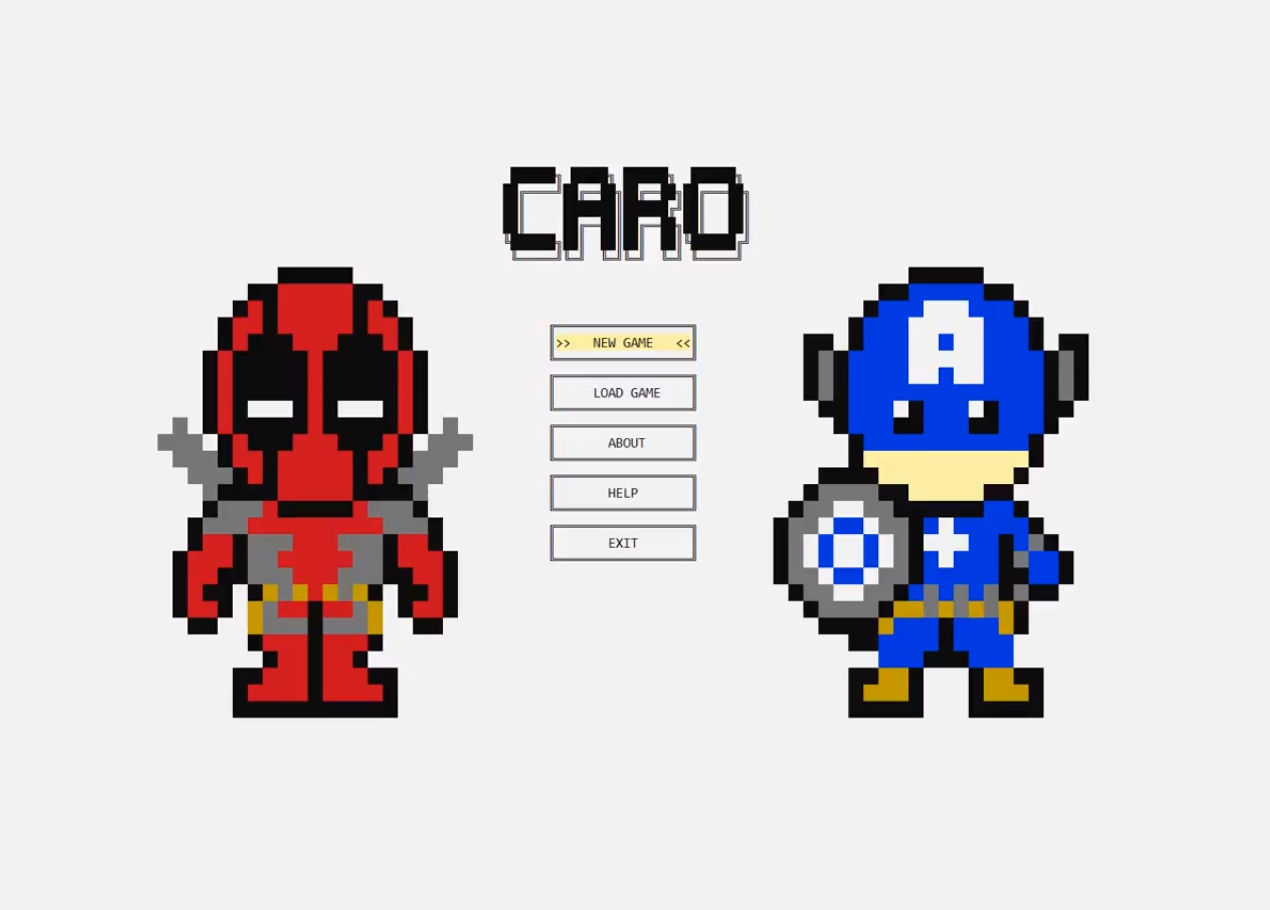
\includegraphics[scale=.5]{img/title.png}
    \caption{Title (updated 17/11/2023)}
\end{figure}
\clearpage
\subsubsection{New Game}
Trong cửa sổ nhỏ New Game, có 2 chế độ để người chơi lựa chọn:
\begin{itemize}
    \item Chơi với máy (1 Player)
    \item Hai người chơi (2 Players)
\end{itemize}
\begin{figure}[H]
    \centering
    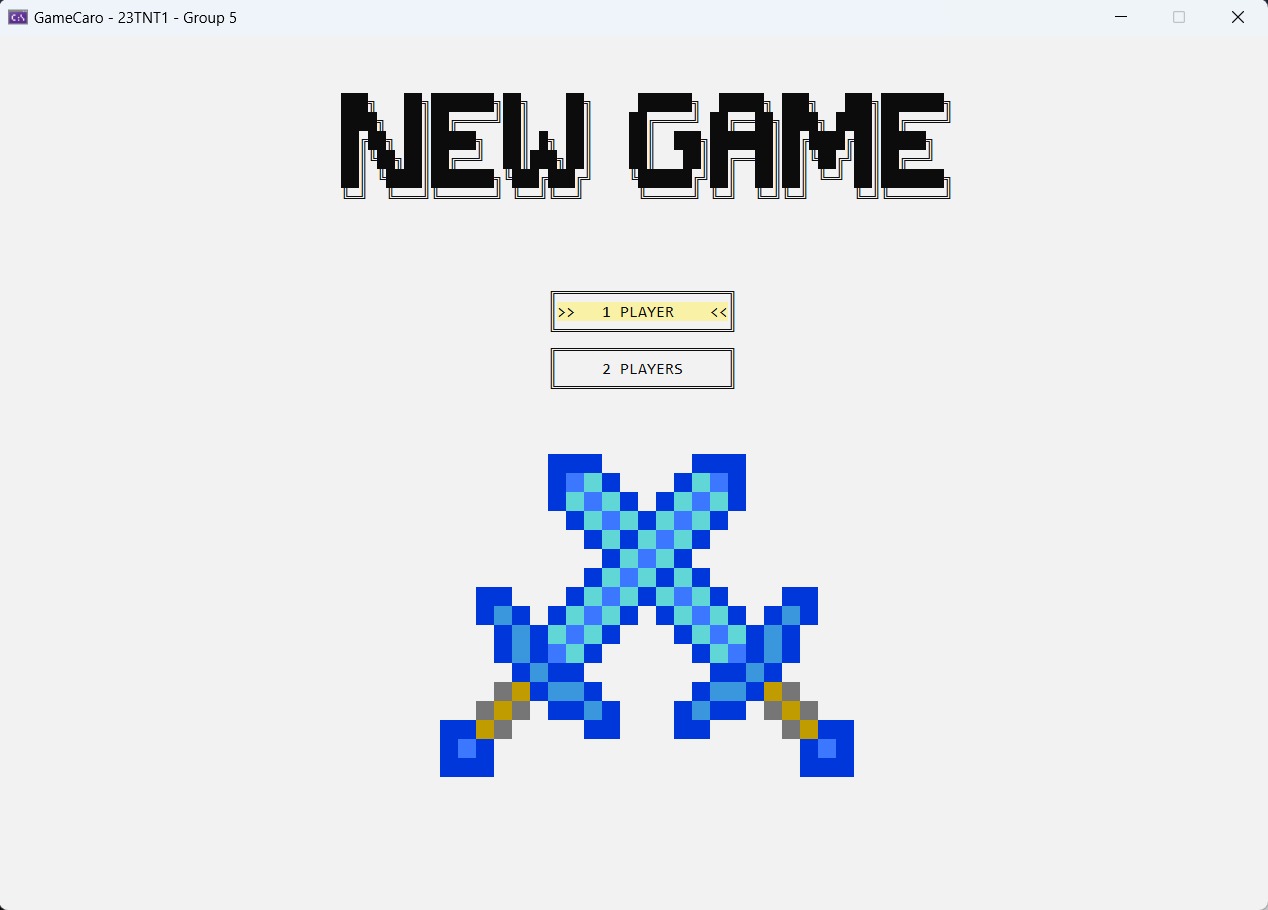
\includegraphics[scale=.4]{img/newgame.png}
    \caption{New Game (updated 17/11/2023)}
\end{figure}
\clearpage
\subsubsection{In match}
Người chơi có thể di chuyển bằng các nút trên bàn phím. Trong quá trình chơi, biểu tượng X và O sẽ thay đổi màu sắc để thông báo lượt đi. Khi phân định thắng-thua, dòng liên tiếp 5 ô X hoặc O sẽ nhấp nháy và kết quả sẽ được hiển thị qua hộp thoại với thông báo "X WIN" hoặc "O WIN". Người chơi cũng có thể lựa chọn các chế độ như "Exit Game" (Esc), "Undo" (U) và "Save Game" (I) trong quá trình chơi.
\begin{figure}[H]
    \centering
    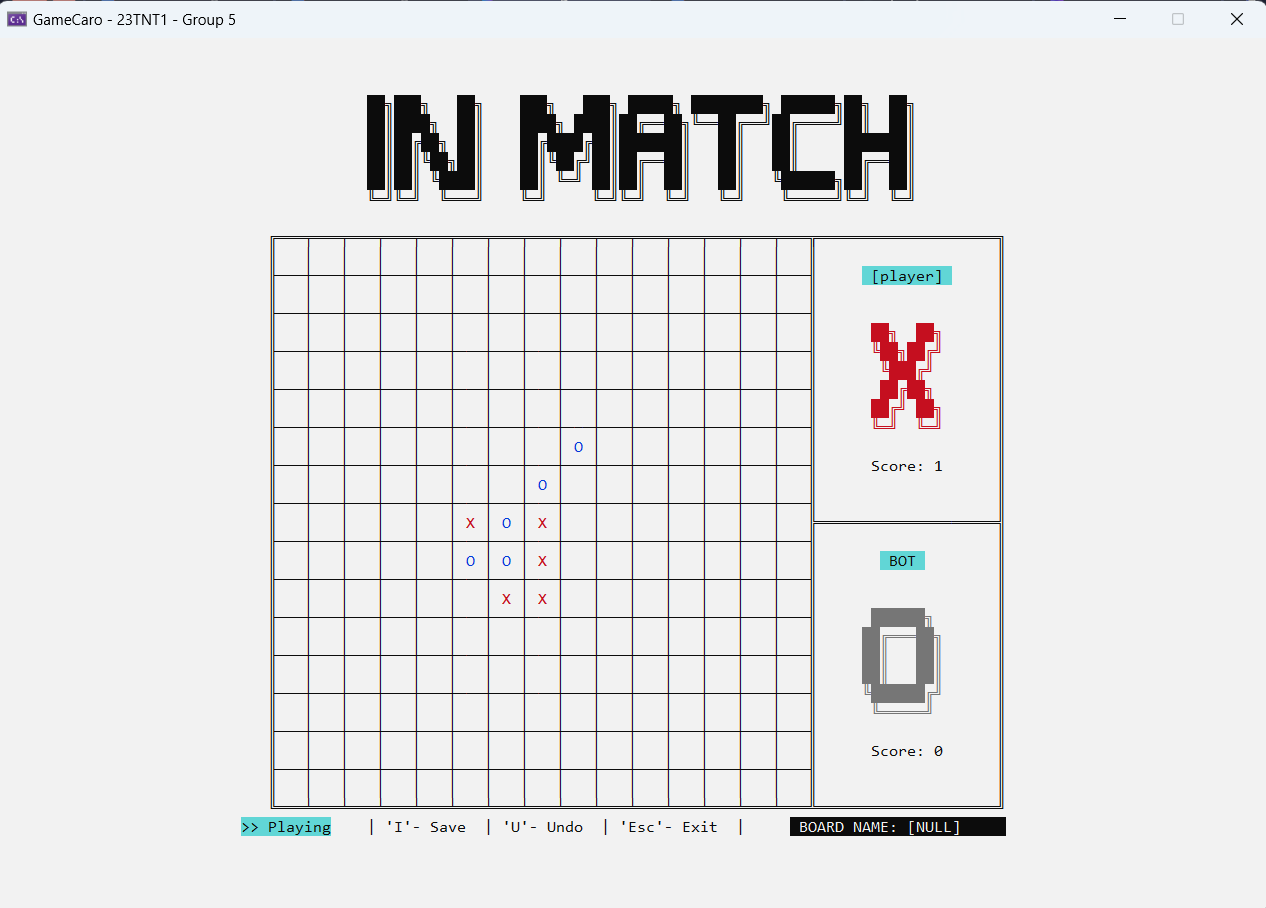
\includegraphics[scale=.4]{img/inmatch.png}
    \caption{In Match (updated 17/11/2023)}
\end{figure}
\clearpage
\subsubsection{Load Game}
Có tổng cộng 15 file trống được cung cấp cho người chơi để thuận tiện trong việc lưu trữ. Mỗi file có một tên và độ dài tên nhất định. Khi người chơi chọn một file đã lưu, họ sẽ có một loạt các lựa chọn, bao gồm "PLAY" (để quay lại màn hình chính và tiếp tục chơi), "DELETE" (để xóa file đã lưu) hoặc "RENAME" (để đổi tên file nếu người chơi muốn thay đổi tên).
\begin{figure}[H]
    \centering
    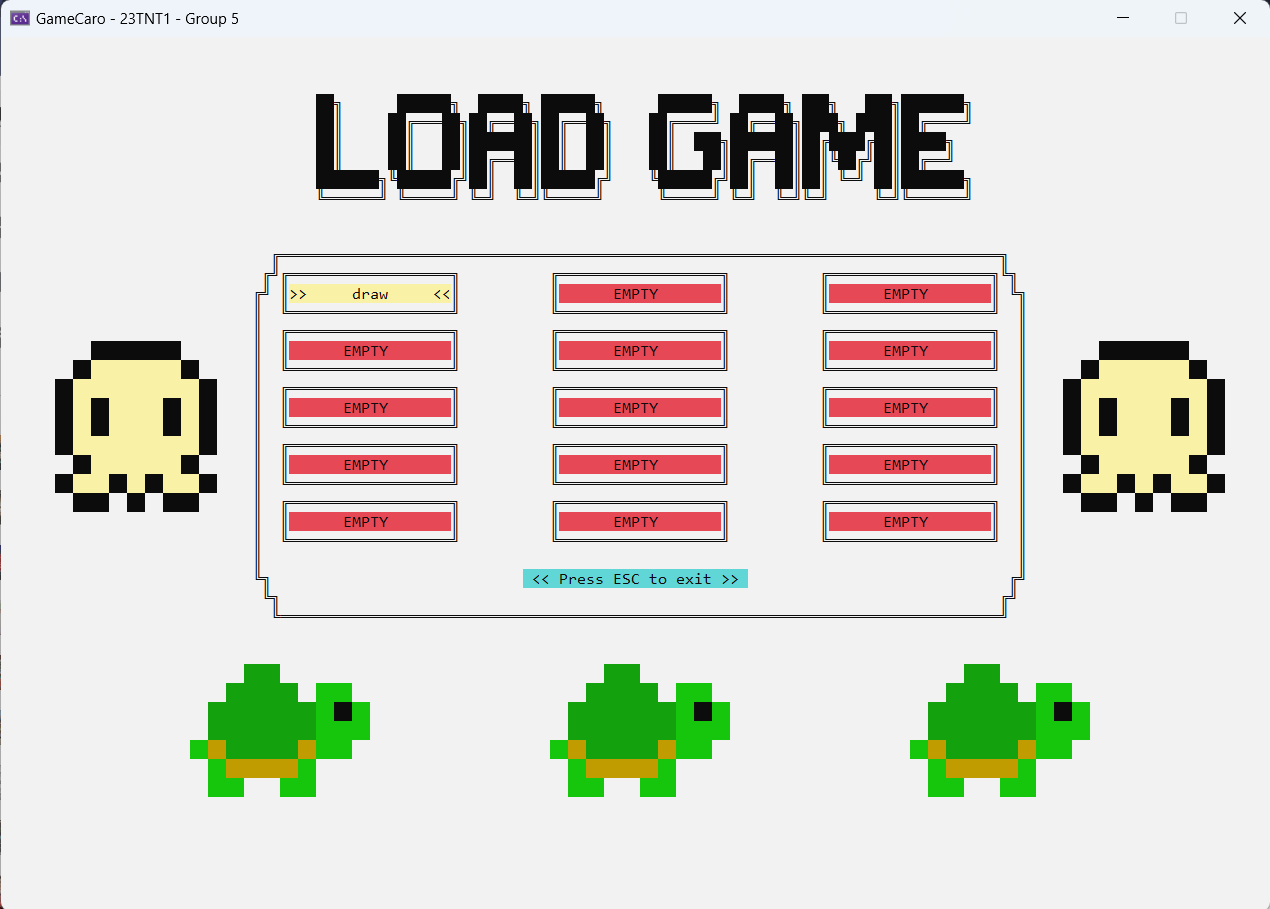
\includegraphics[scale=.4]{img/loadgame.png}
    \caption{Load Game (updated 17/11/2023)}
\end{figure}
\clearpage
\subsubsection{Help}
Phần Help có các hướng dẫn cơ bản cho người chơi.
\begin{figure}[H]
    \centering
    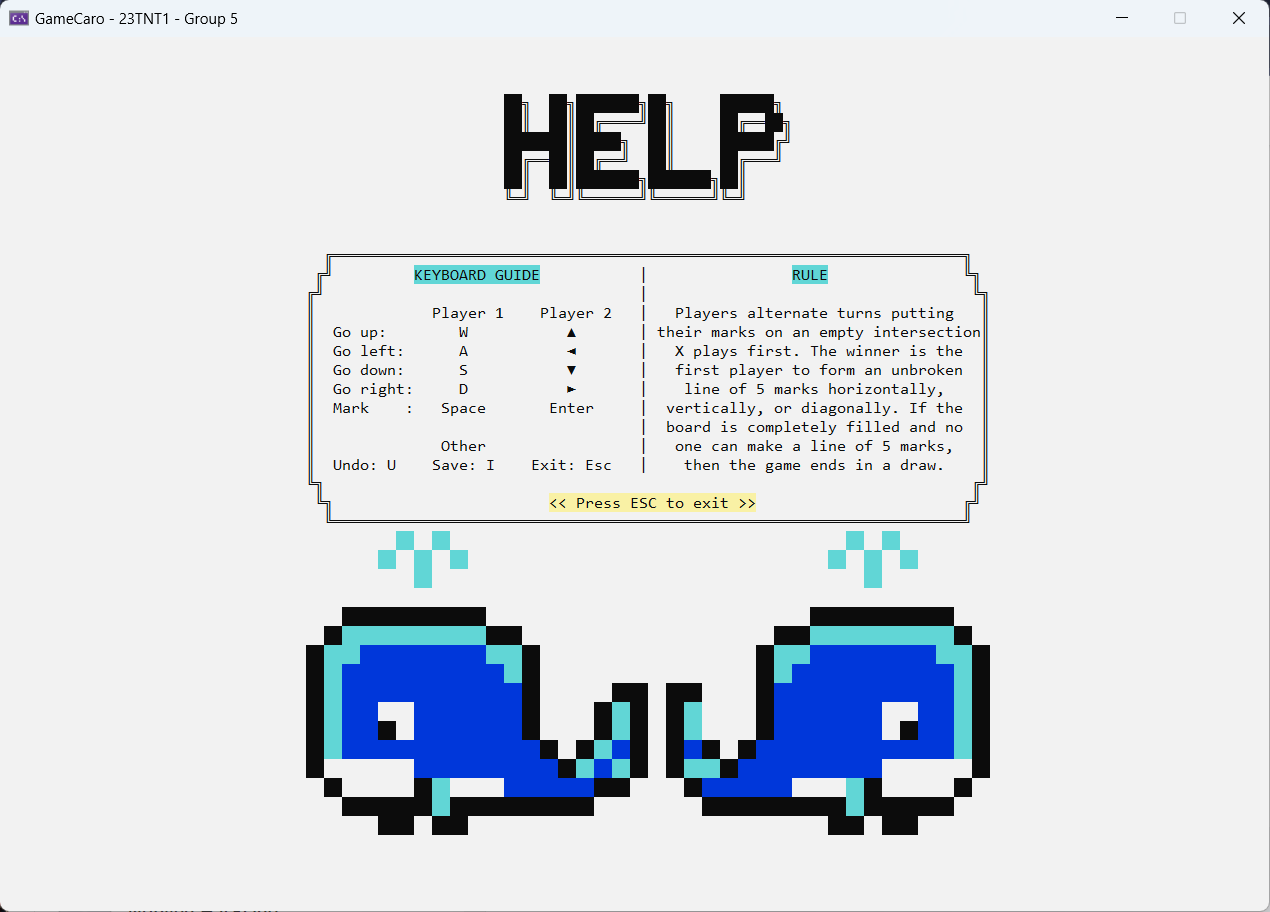
\includegraphics[scale=.4]{img/help.png}
    \caption{Help (updated 17/11/2023)}
\end{figure}
\clearpage
\subsubsection{About}
Phần About gồm thông tin thành viên nhóm và giảng viên hướng dẫn.
\begin{figure}[H]
    \centering
    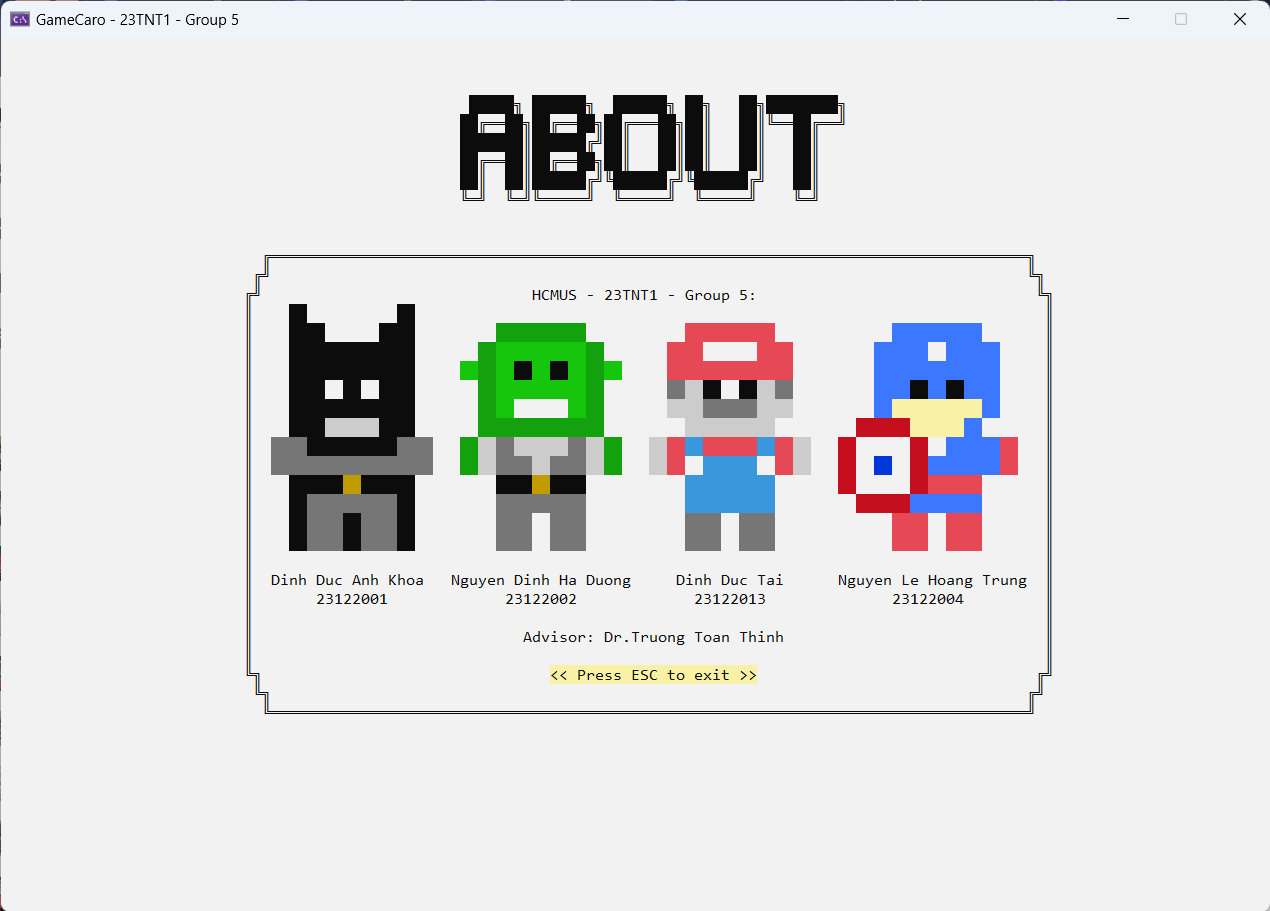
\includegraphics[scale=.4]{img/about.png}
    \caption{About (updated 17/11/2023)}
\end{figure}
\clearpage
\subsection{Thuật toán - Hệ thống trò chơi}
Đây là những chức năng đã được xây dựng thành công, cùng với một phần thuật toán để minh họa:
\subsubsection{Minimax, Alpha-Beta Pruning}
Xây dựng thuật toán AI dành cho chế độ 1 người chơi : Thuật toán Minimax, thuật toán cắt tỉa Alpha-Beta
\lstinputlisting[language=C++]{code/minimax.cpp}
\subsubsection{Điều khiển bằng bàn phím}
Người chơi có thể điều khiển bằng các phím AWDS, các phím mũi tên cùng các phím khác như I, U, Space, Esc,... để tương tác với trò chơi.
\lstinputlisting[language=C++]{code/keyboard.cpp}
\subsubsection{Lưu và chơi tiếp game}
Vào cửa sổ nhỏ Load Game để chơi tiếp trò chơi đã lưu. Trong khi chơi, có thể lưu lại game.
\lstinputlisting[language=C++]{code/saveload.cpp}
\subsubsection{Phân định thắng thua}
Khi hoàn thành trò chơi,hệ thống sẽ phân định thắng thua giữa hai người chơi. 
\lstinputlisting[language=C++]{code/winlose.cpp}
\subsubsection{2 chế độ chơi}
Có 2 chế độ : Đấu với Bot hoặc đấu với người.



\section{Nhận xét - Tổng kết}
\subsection{Nhận xét}
Trong thời gian thực hiện đồ án, các thành viên có tinh thần trách nhiệm và năng lực tốt, hoàn thành nhiệm vụ được giao đúng với thời hạn. Có sự nỗ lực lớn, tinh thần đoàn kết giúp đỡ nhau giữa các thành viên.
\subsection{Tổng kết}
\begin{itemize}
    \item Đồ án hoàn thành đúng tiến độ và có độ hoàn thiện cao.
    \item Các thành viên trong nhóm có tinh thần trách nhiệm, hoàn thành tốt nhiệm vụ được giao.
\end{itemize}
\subsection{Lời cảm ơn}
Nhóm xin chân thành cảm ơn giảng viên - TS. Trương Toàn Thịnh đã hướng dẫn để chúng em có thể hoàn thành tốt được đồ án môn Nhập môn lập trình.\\

Xin cảm ơn các thành viên trong nhóm đã có trách nhiệm và nhiệt tình giúp đỡ nhau, hoàn thành đồ án theo yêu cầu.



%References
\cleardoublepage
\phantomsection
\addcontentsline{toc}{section}{Tài liệu}
\bibliographystyle{plain}
\bibliography{ref/ref} 
\label{thamkhao}

%Appendix
%\appendix
% Add \cleardoublepage to move appendices to next page.
%\section{Phụ lục}
\begin{itemize}
\item Template này \textbf{không phải} là template chính thức của Khoa Công nghệ thông tin - Trường Đại học Khoa học Tự nhiên.
\item Các hình ảnh, bảng biểu, thuật toán trong template chỉ mang tính chất ví dụ.
\item Nhóm tác giả phân phối \textbf{miễn phí} template này \href{https://github.com/khongsomeo/hcmus-unofficial-report-template}{trên GitHub} và \href{https://www.overleaf.com/latex/templates/hcmus-report-template/zyrhmsxynwqs}{trên Overleaf} với \href{https://github.com/khongsomeo/hcmus-unofficial-report-template/blob/main/LICENSE}{Giấy phép GNU General Public License v3.0}. Nhóm tác giả không chịu trách nhiệm với các bản phân phối không nằm trong hai kênh phân phối chính thức nêu trên.
\end{itemize}

\end{document}